\chapter{Путеводитель по параллелизму для путешествующих автостопом}
\label{the-hitchhikers-guide-to-concurrency}
Далеко\--далеко в закоулках нефешенебельного начала 21\--го века, которого даже нет на карте, находится маленькое подмножество человеческих знаний.

В этом подмножестве заключена совершенно невзрачная маленькая дисциплина, чья Фон\--Неймановская архитектура столь примитивна, что согласно ей ОПЗ\--калькуляторы считаются чем\--то выдающимся.

У этой дисциплины есть, а точнее была \--- проблема: большинство людей, изучающих её, были почти всегда недовольны, создавая параллельное ПО.
Предлагалось множество решений этой проблемы, но чаще всего они были связаны с перемещением маленьких логических блоков, которые назывались локами, мутексами и всякими другими именами, что несколько странно, поскольку этим самым блокам параллелизм был совершенно не нужен.

Так проблема и оставалась нерешённой.
Одни люди были озлоблены, другие просто вызывали жалость, и даже ОПЗ\--калькуляторы им не помогали.

Кое\--кто был убеждён, что людям не стоило добавлять параллелизм в языки программирования.
И что программы вообще не должны были выходить из их первоначального потока.
\\
\colorbox{lgray}
{
\begin{minipage}{1.0\linewidth}
    \textbf{Замечание:} неплохое развлечение \--- писать пародии на <<Путеводитель по галактике для путешествующих автостопом>>.
    Если вам ещё не попадалась эта книга, то обязательно её прочтите.
    Она стоит того!
\end{minipage}
}
\section{Без паники}
\label{dont-panic}
\begin{wrapfigure}{l}{0.35\linewidth}
    
\includegraphics[width=1\linewidth]{fat-guy.png}
\end{wrapfigure}
Привет.
Сегодня (или в любой из дней, когда вы читаете эти строки, может быть даже завтра) я хочу рассказать вам о параллельном Erlang.
Скорее всего вы уже читали о параллелизме, или когда\--либо сталкивались с ним.
Может быть, вы интересуетесь истоками программирования для множества ядер, или читаете эту книгу, наслушавшись болтовни, которой в наше время окружён параллелизм.

Впрочем, хочу вас предупредить, что в этой главе основной упор сделан на теорию.
Если у вас болит голова, или вы питаете отвращение к истории языков программирования, или вам просто хотелось попрограммировать, то перейдите лучше к ~\ref{thanks-for-all-the-fish}~концу главы, или сразу к следующей (там как раз освещается более практическая сторона вопроса).

Я уже объяснил во введении к книге, что параллелизм в Erlang основан на передаче сообщений и модели акторов.
Мой пример рассказывал о людях, общение которых происходит исключительно при помощи писем.
Чуть позже я ещё вернусь к этой модели, а сейчас нам необходимо первым делом обозначить разницу между \emph{конкурентностью} и \emph{параллелизмом}.

Оба слова во многих ситуациях имеют одно и то же значение.
Но в контексте Erlang они часто относятся к двум разным концепциям.
По мнению большинства эрлангистов понятие конкурентности описывает несколько акторов, которые исполняются независимо друг от друга, но их исполнение не обязательно происходит в один тот же момент.
Параллелизм же означает, что несколько акторов исполняются одновременно.
Взгляды различных областей computer science на правильность этих определений могут не совпадать, но в этом руководстве я буду пользоваться именно такими определениями.
Не удивляйтесь, если в других источниках вы увидите, как кто\--то употребляет те же самые термины для обозначения других понятий.

Конкурентность была в Erlang с самого начала, даже в восьмедисятые, когда всё запускалось на одноядерном процессоре.
Каждому процессу Erlang для исполнения отводился свой собственный временной отрезок, совсем как в эру десктопных приложений, которая предшествовала появлению многоядерных систем.

Уже в то время можно было, в принципе, реализовать параллелизм.
Для этого нам бы потребовался второй компьютер, который исполнял бы код и обменивался информацией с первым.
Но даже такая система смогла бы исполнять параллельно всего лишь два актора.
Современные многоядерные системы позволяют реализовать параллелизм в рамках одного компьютера (некоторые промышленные чипы могут содержать десятки ядер), и Erlang использует эту возможность в полной мере.\\
\colorbox{lorange}
{
\begin{minipage}{1.0\linewidth}
    \textbf{Не забывайтесь:}\\
    Важно понимать разницу между конкурентностью и параллелизмом.
    Многие программисты верят, что Erlang был готов к использованию на многоядерных компьютерах задолго до того, как это произошло в действительности.
    Erlang стал использовать истинную \href{http://en.wikipedia.org/wiki/Symmetric\_multiprocessing}{симметричную мультипроцессорность} (symmetric multiprocessing) лишь в середине двухтысячных, а большая часть реализации была завершена в релизе R13B в 2009 году.
    До этого часто приходилось отключать SMP, чтобы избежать потерь производительности.
    На многоядерном компьютере без SMP можно получить параллелизм, если запустить одновременно несколько экземпляров виртуальной машины.\\
    \\
    Интересно отметить, что для внесения истинного параллелизма в язык, не потребовалось производить какие\--либо концептуальные изменения на языковом уровне.
    Благодаря тому, что конкурентность в Erlang строится вокруг изолированных процессов, все изменения были сделаны внутри VM, подальше от глаз обычного программиста.
\end{minipage}
}
\section{Принципы конкурентности}
\label{concepts-of-concurrency}
\begin{wrapfigure}{r}{0.35\linewidth}
    
\includegraphics[width=1\linewidth]{erlang-the-movie.png}
\end{wrapfigure}
Когда\--то разработка языка Erlang проходила в быстром темпе, и от инженеров, которые занимались разработкой на Erlang для телефонных коммутаторов, поступал плотный поток обратной связи.
Их отчёты подтвердили, что конкурентность, основанная на процессах, и асинхронная передача сообщений позволяли хорошо моделировать задачи, возникающие перед разработчиками.
Кроме того, ещё до появления Erlang, в мире телефонии уже сформировалась некая культура, тяготеющая к параллелизму.
Она была унаследована от языка PLEX, который ранее был создан в Ericsson, и использовался в коммутаторах AXE.
Erlang унаследовал эту тенденцию, и попытался усовершенствовать существующие инструменты.

Для того, чтобы Erlang считался хорошим инструментом, он должен был удовлетворять нескольким требованиям.
Главным условием была возможность масштабирования и поддержки тысяч и тысяч пользователей на множестве коммутаторов.
Также эти коммутаторы должны были обеспечивать высокую надёжность работы \--- вплоть до того, что исполнение кода никогда не должно было останавливаться.

\subsection{Масштабируемость}
\label{scalability}
Для начала я расскажу о масштабировании.
Для достижения масштабируемости была необходима система, обладающая определёнными свойствами.
В такой системе пользователи были бы представлены при помощи процессов, которые реагируют на определённые события (например, приём звонка, завершение разговора и т.д.).
Идеальная система должна поддерживать процессы, выполняющие малые объёмы вычислений, и быстрое переключение между процессами при поступлении событий. 
Высокоэффективная обработка процессов предполагала возможность их очень быстрого старта, очень быстрого уничтожения, и очень быстрой коммутации.
Обязательным условием для такого поведения была легковесность процессов.
Это было также необходимо, чтобы избавиться от наличия пула процессов (фиксированное множество процессов, между которыми распределяется работа).
Намного легче создавать программы, которые используют сразу столько процессов, сколько нужно.

Ещё один важный аспект масшабируемости \--- это возможность преодоления ограниченности ресурсов оборудования.
Для решения этой задачи выделяют два направления: можно улучшать характеристики оборудования, а можно увеличивать его количество.
Первое решение будет работать до определённого момента, после которого за улучшение придётся очень дорого платить (необходимо, например, покупать суперкомпьютер).
Второе решение, как правило, обходится дешевле.
Для выполнения тех же задач нужно просто добавлять больше компьютеров.
Вот где вашему языку может пригодиться распределённость.

Вернёмся к обсуждению лёгких процессов.
Высокая надёжность очень важна для нужд телефонии, поэтому разработчики решили, что правильнее всего будет запретить процессам иметь общую память.
Некоторые аварийные ситуации с участием разделяемой памяти могут привести к противоречивому состоянию (особенно если данные разделяются между несколькими узлами) и осложнениям.
Вместо этого процессы должны общаться при помощи сообщений, которые содержат полные копии данных.
Этим мы рискуем получить более медленное, но зато более надёжное решение.
\subsection{Устойчивость к сбоям}
\label{fault-tolerance}
Мы приходим ко второму требованию, которому должен соответствовать Erlang: надёжность.
Первые разработчики на Erlang всегда помнили о том, что сбои происходят повсеместно.
Можно сколько угодно пытаться предотвратить ошибки, но в большинстве случаев от некоторых из них не получится избавиться полностью.
И даже если не будет ошибок \--- от сбоев оборудования никуда не денешься.
Поэтому вместо того, чтобы пытаться полностью предотвратить ошибки, лучше найти хороший способ их обрабатывать.

Оказывается, что подход к проектированию при помощи множественных процессов с передачей сообщений, оказался верным, так как в него можно относительно легко встроить обработку ошибок.
Возьмём, к примеру, легковесные процессы (созданные для быстрых перезапусков и выключений).
Исследования показали, что для масштабных программных комплексов главным источником простоя являются ошибки, которые нерегулярно себя проявляют и спонтанно исчезают (\href{http://dslab.epfl.ch/pubs/crashonly/}{источник}).
Существует правило, говорящее что ошибки, которые искажают данные, должны как можно быстрее приводить к остановке неисправной части системы, чтобы предотвратить проникновение ошибок и плохих данных в остальные узлы.
Есть также ещё одна концепция, согласно которой существует множество различных способов остановки системы.
Двумя такими способами являются корректная остановка и сбой (завершение, вызванное непредвиденной ошибкой).

Очевидно, что наихудшим исходом будет сбой.
Для надёжного устранения проблемы сбоев можно сделать так, чтобы все аварийные ситуации проходили так же, как и корректные остановки.
Для этого необходимо использовать ряд методов, к которым можно отнести принцип неразделяемости ресурсов (shared-nothing) и единичное присваивание (single assignment) (которое позволяет изолировать память процесса), уход от \href{http://en.wikipedia.org/wiki/Lock_(computer_science)}{блокировок} (после аварии блокировка может остаться закрытой, и будет перекрывать другим процессам доступ к данным, или просто приводить данные в нестабильное состояние), а также другие техники, которые я не буду подробно описывать, но они также использовались при проектировании Erlang.
Таким образом, идеальным решением аварийной ситуации в Erlang считается быстрое уничтожение процессов, которое позволяет избежать порчи данных и случайных, нерегулярных ошибок.
Ключевым элементом этой схемы являются лёгкие процессы.
В языке также присутствуют механизмы обработки ошибок, которые позволяют процессам следить за другими процессами (подробнее о них в главе \ref{errors-and-processes}~Ошибки и процессы), определять момент смерти процесса и планировать действия, связанные с этим событием.

Предположим, что быстрый перезапуск процессов позволил нам справиться с аварийными ситуациями.
Следующая проблема \--- сбои оборудования.
Как же сделать так, чтобы программа работала даже тогда, когда кто\--то пинает ногами компьютер, на котором она запущена?
Сложнейший защитный механизм, состоящий из лазерных детекторов и стратегически расставленных кактусов, конечно же, проработает какое\--то время, но надолго его не хватит.
Напрашивается мысль, что можно просто запустить программу сразу на нескольких компьютерах.
Ведь мы это и так уже делаем при масштабировании.
Вот вам и ещё одно преимущество независимых процессов, единственным средством коммуникации которых является передача сообщений.
Они будут работать одинаково и на локальном и на удалённом компьютере.
Такая отказоустойчивость посредством распределённости будет работать практически без участия программиста.
\begin{wrapfigure}{l}{0.35\linewidth}
    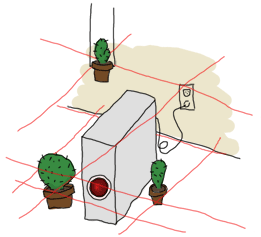
\includegraphics[width=1\linewidth]{cacti-laser.png}
\end{wrapfigure}

Распределённость напрямую влияет на общение процессов между собой.
Мы не можем быть уверены, что если узел (удалённый компьютер) существовал в момент вызова функции, то он будет существовать и во время передачи вызова, и что вызов вообще будет правильно выполнен.
Это одно из самых серьёзных препятствий для внедрения распределённости.
Если кто\--то споткнётся о кабель питания или выключит компьютер, то ваше приложение зависнет.
А может быть оно аварийно завершится.
Кто знает?

Выбор асинхронной передачи сообщений, оказывается, тоже был верным шагом.
Cогласно модели "процессы с асинхронной передачей сообщений", сообщения передаются от одного процесса к другому и хранятся в почтовом ящике принимающего процесса до тех пор, пока они не будут извлечены и прочитаны.
При отсылке сообщения мы даже не проверяем, что получающий процесс существует, так как пользы от этой проверки нет никакой.
Как сказано в предыдущем абзаце, невозможно узнать заранее, что за время, прошедшее между отсылкой сообщения и его получением, не случится аварийное завершение процесса.
А если сообщение всё же получено, то невозможно узнать, что процесс\--получатель хоть как\--то отреагирует на сообщение, или вообще доживёт до этого момента.
Асинхронные сообщения позволяют безопасно вызывать удалённые функции, так как не делают никаких прогнозов о возможном развитии событий.
Прогнозы  должен делать программист.
Если вам нужно подтвердить факт доставки, то в ответ необходимо послать оригинальному процессу подтверждающее сообщение.
Для сообщения, а также для любой программы или библиотеки, построенной на этом принципе, будут выполняться те же самые принципы безопасности.
\subsection{Реализация}
\label{implementation}
В общем, было принято решение, что легковесные процессы с асинхронной передачей сообщений полностью подходят Erlang.
Как теперь всё это заставить работать?
Ну, во\--первых, нельзя доверять операционной системе управление процессами.
Операционные системы имеют слишком много методов регуляции процессов, причём эти методы очень сильно различаются по своей производительности.
Большинство методов, если не все, слишком медленны или слишком тяжелы для нужд стандартных областей применения Erlang.
Перенося эти механизмы регуляции внутрь VM, разработчики Erlang сохраняют контроль над оптимизацией и надёжностью.
Современный процесс Erlang занимает около 300 слов памяти, и может создаваться за микросекунды.
В большинстве сегодняшних операционных систем такое не увидишь.

\begin{wrapfigure}{r}{0.35\linewidth}
    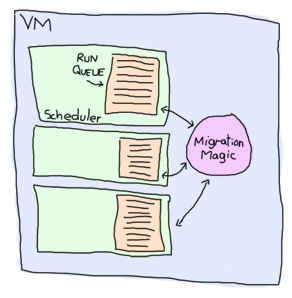
\includegraphics[width=1\linewidth]{schedulers.png}
\end{wrapfigure}
Чтобы справляться с множеством потенциальных процессов, которые может создать ваша программа, VM создаёт по одному потоку на каждое ядро.
Эти потоки будут выполнять функцию \emph{планировщика} (scheduler).
Каждый планировщик обслуживает \emph{очередь исполнения} (run queue), которая представляет собой список процессов Erlang, между которыми распределяются отрезки времени.
Когда в очереди исполнения какого\--либо из планировщиков появляется слишком много задач, часть из них переносят в другую очередь.
Так что каждая виртуальная машина Erlang самостоятельно осуществляет балансировку нагрузки, и программиста это не должно беспокоить.
Выполняются также и другие оптимизации, например ограничение частоты отсылки сообщений перегруженным процессам, что позволяет регулировать и перераспределять нагрузку.

Всё самое сложное будет делать вместо вас вирутальная машина.
Именно благодаря этой автоматизации в Erlang можно легко перейти к параллельному исполнению задач.
Переход к параллельному исполнению означает, что скорость работы вашей программы возрастёт в два раза, если вы добавите второе вычислительное ядро, в четыре раза, если добавить ещё 4 и так далее, правильно?
Не всегда.
Такой рост скорости, зависящий от количества ядер или процессоров, называется \emph{линейным масштабированием} (linear scaling) (см. график ниже).
К сожалению, в реальности не бывает бесплатных обедов (бывают на похоронах, но за них всё равно кто\--то платит).
\section{Почти линейное масштабирование, но не совсем}
\label{not-entirely-unlike-linear-scaling}
Линейное масштабирование трудно осуществлять не из\--за самого языка, а из\--за природы решаемых задач.
О задачах, которые очень хорошо масштабируются, иногда говорят, что они \emph{очевидно  параллельны} (embarassingly parallel).
Если вы поищете в Интернет очевидно параллельные задачи, то скорее всего наткнётесь на примеры алгоритмов трассировки лучей (ray\--tracing) (метод создания 3D изображений), поиска грубой силой в криптографии, предсказания погоды и т.д.

Время от времени на IRC каналах, форумах или почтовых рассылках появляются люди с вопросом, можно ли применять Erlang для решения таких задач, и можно ли при этом использовать \href{http://en.wikipedia.org/wiki/Graphics_Processing_Unit}{GPU}.
Ответ на этот вопрос почти всегда отрицательный, и причина для этого сравнительно проста: все эти задачи обычно решаются при помощи численных алгоритмов, перемалывающих большие объёмы данных.
Erlang справляется с такими задачами не очень хорошо.

Задачи, которые являются очевидно параллельными для Erlang, относятся к более высокому логическому уровню.
Обычно они связаны с такими понятиями как чат\--серверы, телефонные коммутаторы, веб\--серверы, очереди сообщений, поисковые роботы, ну или любые другие задачи, в которых действия могут быть представлены как независимые логические элементы (кто\--нибудь вспомнил об акторах?).
Такой тип задач можно эффективно решать с масштабированием, приближающимся к линейному.

Но для некоторых задач такие характеристики масштабирования недостижимы.
Если в решении присутствует одна централизованная последовательность операций, то о линейности масштабирования можно забыть.
\textbf{Ваша параллельная программа не может работать быстрее, чем её самая медленная последовательная часть.}
Пример такого феномена можно наблюдать при любом походе в супермаркет.
Сотни людей могут одновременно выбирать товары в зале, при этом почти не мешая друг другу.
Но если количество покупателей превышает число кассиров, то при оплате покупок сразу образуются очереди.

Можно было бы добавлять кассиров до тех пор, пока на каждого покупателя не будет приходиться по одному кассиру, но тогда вам придётся для каждого покупателя добавлять и собственную дверь, потому что они не смогут все одновременно входить и выходить из магазина.

Иначе говоря, хоть покупатели и могли выбирать необходимые товары параллельно, и это отнимало бы столько же времени, сколько нужно для выбора товаров в одиночестве, но в конце концов им всё равно пришлось бы ожидать своей очереди на пути к кассе.

В обобщённом виде этот принцип называется \href{http://en.wikipedia.org/wiki/Amdahl\%27s_law}{законом Амдала}.
Он демонстрирует ускорение, которое можно ожидать от системы после добавления параллелизма, учитывая соотношение объёма параллельного и последовательного кода:

\begin{figure}[h!]
    \centering
    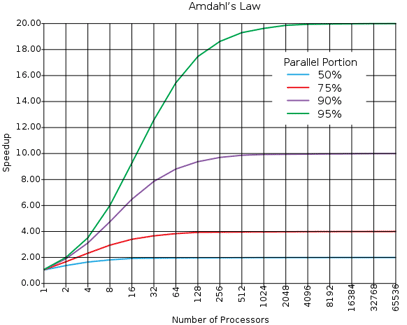
\includegraphics[width=0.7\textwidth]{amdahl.png}
\end{figure}
Согласно закону Амдала, код параллельный на 50\% никогда не сможет стать быстрее более чем в два раза, а код параллельный на 95\% теоретически может работать в 20 раз быстрее, при наличии достаточного количества процессоров.
Интересно видеть на этом графике, что удаление последних непараллельных частей программы теоретически даст огромный прирост скорости, по сравнению с удалением последовательного кода из программы, которая и до удаления была не очень\--то параллельной.\\
\colorbox{lorange}
{
\begin{minipage}{1.0\linewidth}
    \textbf{Не забывайтесь:}\\
    Параллелизмом \emph{не получится} решить любую проблему.
    В некоторых случаях добавление параллелизации замедлит ваше приложение.
    Это может произойти, если ваша программа на 100\% состоит из последовательного кода, но при этом пытается использовать несколько процессов.\\
    \\
    Одним из лучших примеров такого поведения является \emph{кольцевой тест} (ring benchmark).
    В этом тесте несколько тысяч процессов последовательно по кругу передают друг другу данные.
    Это очень похоже на \href{http://en.wikipedia.org/wiki/Telephone_game}{игру в телефон}, если такая аналогия вам покажется знакомой.
    В этом тесте в каждую единицу времени лишь один процесс выполняет полезную работу, но виртуальная машина Erlang в это время всё равно не прекращает распределять нагрузку между ядрами, и отдаёт каждому процессу положенную ему часть времени.\\
    \\
    Такая ситуация оказывает негативный эффект на множество оптимизаций, применяемых в оборудовании, и заставляет виртуальную машину тратить время на бесполезные вычисления.
    Зачастую это приводит к тому, что приложение, полностью состоящее из последовательного кода, исполняется на нескольких ядрах значительно медленнее, чем на одном.
    В таком случае не помешает отключить симметричную мультипроцессорность (\ops{\$ erl -smp disable}).
\end{minipage}
}
\section{Прощайте, и спасибо за рыбку!}
Эту глава не была бы полна без рассказа о трёх базовых компонентах, необходимых для осуществления конкурентности в Erlang: создание новых процессов, отсылка сообщений и получение сообщений.
Есть ещё и другие механизмы, необходимые для создания по\--настоящему надёжных приложений, но на данном этапе будет довольно перечисленных.

В своём рассказе я много раз обходил стороной объяснение сущности процесса.
Он является ни чем иным, как функцией.
Вот и всё объяснение.
Запускается функция, и, как только она завершает исполнение, процесс исчезает.
Формально, у процесса есть скрытое состояние (к нему относится, например, ящик для почтовых сообщений), но на данный момент нам будет достаточно обсуждения функций.

Новые процессы в Erlang создаются функцией \ops{spawn/1}, которая принимает в качестве параметра ещё одну функцию и запускает её.
\begin{lstlisting}[style=erlang]
1> F = fun() -> 2 + 2 end.
#Fun<erl_eval.20.67289768>
2> spawn(F).
<0.44.0>
\end{lstlisting}

\ops{spawn/1} возвращает результат (\ops{<0.44.0>}), который называется \emph{идентификатором процесса} (process identifier), и чаще всего именуется сообществом как \emph{PID}, \emph{Pid} или \emph{pid}.
Идентификатор процесса является произвольным значением, которое представляет любой процесс, существующий (или существовавший) в какой\--либо момент жизни виртуальной машины.
Его используют как адрес, необходимый для общения с процессом.

Вы, должно быть, заметили, что мы не видим результат вычисления функции \emph{F}.
Мы получаем лишь pid.
Так происходит потому, что процессы ничего не возвращают.

Как же нам в таком случае увидеть результат выполнения F?
Есть два способа.
Проще всего просто отобразить полученный результат:
\begin{lstlisting}[style=erlang]
3> spawn(fun() -> io:format("~p~n",[2 + 2]) end).
4
<0.46.0>
\end{lstlisting}

Для настоящих программ это не очень удобно, но так мы сможем получить представление об организации процессов в Erlang.
К счастью, для экспериментов, нам будет достаточно функции \ops{io:format/2}.
Мы быстро создадим 10 процессов и приостановим их выполнение на некоторый период времени при помощи функции \ops{timer:sleep/1}.
Она  принимает целое значение \emph{N}, ожидает пока пройдут \emph{N} миллисекунд и продолжает выполнение кода.
После задержки на экран выводится переданное процессу значение.
\begin{lstlisting}[style=erlang]
4> G = fun(X) -> timer:sleep(10), io:format("~p~n", [X]) end.
#Fun<erl_eval.6.13229925>
5> [spawn(fun() -> G(X) end) || X <- lists:seq(1,10)].
[<0.273.0>,<0.274.0>,<0.275.0>,<0.276.0>,<0.277.0>,
<0.278.0>,<0.279.0>,<0.280.0>,<0.281.0>,<0.282.0>]
2  
1  
4  
3  
5  
8  
7  
6  
10 
9 
\end{lstlisting}

Откуда же взялся такой порядок чисел?
Добро пожаловать в параллелизм.
Порядок процессов невозможно гарантировать, так как все процессы стартуют одновременно.
Виртуальная машина Erlang использует множество ухищрений для определения момента запуска того или иного процесса, чтобы каждому процессу гарантированно хватило времени для старта.
Множество сервисов в Erlang реализовано в виде процессов, включая оболочку, в которой вы вводите команды.
Системе приходится балансировать между вашими процессами и процессами, которые необходимы ей самой.
Это может явиться причиной странного порядка запускаемых процессов.\\
\colorbox{lgray}
{
\begin{minipage}{1.0\linewidth}
    \textbf{Замечание:} если включить или отключить симметричное мультипроцессирование, то результаты не будут сильно отличаться.
    Можете сами в этом убедиться, запустив виртуальную машину Erlang командой \ops{\$ erl -smp disable}.\\
    \\
    Чтобы узнать, используется ли SMP в запущенной виртуальной машине, запустите новую VM без каких\--либо параметров и обратите внимание на первую выведенную строку.
    Если вы видите там такой текст: [smp:2:2] [rq:2], то в вашей виртуальной машине включена поддержка SMP, и 2 очереди исполнения (rq, или планировщики) работают на двух ядрах.
    Если вы видите только [rq:1], то поддержка SMP отключена.\\
    \\
    Знайте \--- [smp:2:2] означает, что вам доступны два ядра с двумя планировщиками.
    [rq:2] означает, что активны две очереди исполнения.
    В более ранних версиях Erlang можно было иметь множество планировщиков, но у всех у них была единственная общая очередь исполнения.
    Начиная с версии R13B, по умолчанию для каждого планировщика выделяется своя очередь исполнения.
    Это способствует улучшению параллелизма.
\end{minipage}
}

Я хочу доказать вам, что оболочка реализована как обычный процесс, и для этого я буду использовать встроенную функцию \ops{self/0}, которая возвращает pid текущего процесса:
\begin{lstlisting}[style=erlang]
6> self().
<0.41.0>
7> exit(self()).
** exception exit: <0.41.0>
8> self().
<0.285.0>
\end{lstlisting}
pid поменялся из\--за перезапуска процесса.
Подробности работы этого механизма мы рассмотрим позже.
А сейчас нам необходимо разобраться в более простых вещах.
Первым делом рассмотрим, как пересылать сообщения, ведь никому не хочется постоянно выводить результаты работы процессов на экран, а затем вручную вводить их в других процессах (по крайней мере, я это делать совершенно точно не хочу).

Для пересылки сообщений нам понадобится следующий элемент: оператор \ops{!\strut}, известный также как \emph{bang}\--символ.
Слева он принимает в качестве параметра pid процесса, а справа должен находиться любой терм Erlang.
Затем указанный терм пересылается процессу, который обозначен указанным pid, и тот получает к терму доступ:
\begin{lstlisting}[style=erlang]
9> self() ! hello.
hello
\end{lstlisting}

Сообщение уже попало в почтовый ящик процесса, но ещё не было прочитано.
Второе \ops{hello} это значение, возвращённое операцией отсылки.
Таким способом можно отправлять одно и то же сообщение сразу нескольким процессам:
\begin{lstlisting}[style=erlang]
10> self() ! self() ! double.
double
\end{lstlisting}

Эта запись эквивалентна выражению \ops{self() ! (self() ! double)}.
Нужно сделать ремарку насчёт почтового ящика процесса: сообщения хранятся в ящике в том порядке, в котором они были получены.
Для прочтения каждое сообщение извлекается из ящика.
Опять же, этот процесс немного напоминает пример из введения, рассказывающий о людях, которые пишут друг другу письма.
\begin{figure}[h!]
    \centering
    
\includegraphics[width=0.7\textwidth]{hello.png}
\end{figure}

Вы можете использовать в оболочке команду \ops{flush()} для просмотра содержимого текущего почтового ящика:
\begin{lstlisting}[style=erlang]
11> flush().
Shell got hello
Shell got double
Shell got double
ok
\end{lstlisting}

Эта функция \--- просто средство для вывода полученных сообщений.
То есть, поместить результат работы процесса в переменную мы всё равно не сможем, но теперь мы хотя бы знаем как отослать сообщение процессу, а потом проверить, что оно получено.

От пересылки сообщений, которые никто не прочитает, толку столько же, сколько от написания эмо\--поэзии, то есть не очень много.
Вот почему нам нужно выражение \ops{receive}.
Не будем слишком долго рассиживаться в оболочке \--- напишем  \href{http://learnyousomeerlang.com/static/erlang/dolphins.erl}{короткую программу} о дельфинах, используя новую конструкцию:
\begin{lstlisting}[style=erlang]
-module(dolphins).
-compile(export_all).
 
dolphin1() ->
    receive
        do_a_flip ->
            io:format("How about no?~n");
        fish ->
            io:format("So long and thanks for all the fish!~n");
        _ ->
            io:format("Heh, we're smarter than you humans.~n")
    end.
\end{lstlisting}

Как видите, \ops{receive} похожа синтаксически на \ops{case\ldots of}.
И они даже работают совершенно одинаково, за исключением того, что receive связывает не выражения между \ops{case} и \ops{of}, а переменные, извлечённые из сообщений.
В receive можно использовать стражи:
\begin{lstlisting}[style=erlang]
receive
    Pattern1 when Guard1 -> Expr1;
    Pattern2 when Guard2 -> Expr2;
    Pattern3 -> Expr3
end
\end{lstlisting}

Теперь этот модуль можно скомпилировать, запустить и начать переговоры с дельфинами:
\begin{lstlisting}[style=erlang]
11> c(dolphins).
{ok,dolphins}
12> Dolphin = spawn(dolphins, dolphin1, []).
<0.40.0>
13> Dolphin ! "oh, hello dolphin!".
Heh, we're smarter than you humans.
"oh, hello dolphin!"
14> Dolphin ! fish.               
fish
15>
\end{lstlisting}

Здесь мы знакомимся с новым способом создания процессов при помощи \ops{spawn/3}.
Эта модификация spawn принимает не одну функцию, а модуль, функцию и её аргументы.
После запуска функции происходит следующее:
\begin{enumerate}
    \item Исполнение доходит до выражения \ops{receive}.
Так как почтовый ящик процесса пуст, наш дельфин ждёт появления сообщения;
\item Получено сообщение <<oh, hello dolphin!>>.
Функция пытается провести сопоставление с образцом \ops{do\_a\_flip}.
Сопоставление не удаётся, и происходит попытка сопоставления с \ops{fish}, которая тоже заканчивается неудачей.
Наконец, сообщение доходит до универсального шаблона (\ops{\strut\_}) и сопоставление завершается удачно.
\item Процесс выводит сообщение <<Heh, we're smarter than you humans.>>
\end{enumerate}

Необходимо заметить, что если первое посланное нами выражение сработало, то на второе процесс \ops{<0.40.0>} никак не отреагировал.
Это произошло из\--за того, что после вывода <<Heh, we're smarter than you humans.>> наша функция завершилась, а вместе с ней завершился и процесс.
Придётся нам перезапустить дельфина:
\begin{lstlisting}[style=erlang]
8> f(Dolphin).   
ok
9> Dolphin = spawn(dolphins, dolphin1, []).
<0.53.0>
10> Dolphin ! fish.
So long and thanks for all the fish!
fish
\end{lstlisting}

И на этот раз сообщение о рыбе срабатывает.
Но ведь было бы полезнее, если бы мы вместо вывода посредством функции \ops{io:format/2} могли получить от дельфина ответ?
Конечно, да! (зачем я вообще спрашиваю?)
Чуть раньше в этой главе я упомянул, что мы можем узнать, получил ли процесс наше сообщение, только если он пошлёт нам ответное.
Нашему дельфиньему процессу нужно знать кому отвечать.
Всё как на почте.
Если мы хотим, чтобы адресат нам ответил, нужно сообщить ему наш адрес.
В рамках Erlang это осуществляется путём упаковки pid процесса в кортеж.
В результате получается сообщение, которое выглядит примерно так: \ops{\{Pid, Message\}}.
Давайте создадим новую функцию\--дельфина, которая будет принимать такие сообщения:
\begin{lstlisting}[style=erlang]
dolphin2() ->
    receive
        {From, do_a_flip} ->
            From ! "How about no?";
        {From, fish} ->
            From ! "So long and thanks for all the fish!";
        _ ->
            io:format("Heh, we're smarter than you humans.~n")
    end.
\end{lstlisting}

Как видите, мы больше не принимаем сообщения \ops{do\_a\_flip}  и \ops{fish}. Теперь мы ожидаем переменную \emph{From}.
Именно там будет находиться идентификатор процесса.
\begin{lstlisting}[style=erlang]
11> c(dolphins).
{ok,dolphins}
12> Dolphin2 = spawn(dolphins, dolphin2, []).
<0.65.0>
13> Dolphin2 ! {self(), do_a_flip}.         
{<0.32.0>,do_a_flip}
14> flush().
Shell got "How about no?"
ok
\end{lstlisting}

Вроде бы работает неплохо.
Мы можем получать ответы на посылаемые нами сообщения (к каждому сообщению мы должны прикладывать свой адрес), но нам всё так же приходится стартовать новый процесс для каждого вызова.
Эту проблему мы можем решить при помощи рекурсии.
Нам нужна функция, которая будет бесконечно вызывать саму себя и постоянно ожидать прихода сообщений.
Эту задачу будет реализовывать \ops{dolphin3/0}:
\begin{lstlisting}[style=erlang]
dolphin3() ->
    receive
        {From, do_a_flip} ->
            From ! "How about no?",
            dolphin3();
        {From, fish} ->
            From ! "So long and thanks for all the fish!";
        _ ->
            io:format("Heh, we're smarter than you humans.~n"),
            dolphin3()
    end.
\end{lstlisting}

В этом примере и универсальное условие, и \ops{do\_a\_flip} входят в цикл при помощи \ops{dolphin3/0}.
Заметьте, что функция оптимизируется в хвостовую рекурсию, и стек она раздувать не будет.
Процесс\--дельфин будет находиться в бесконечном цикле, пока ему будут приходить только эти сообщения, 
Но как только мы пошлём ему сообщение \ops{fish}\--- процесс сразу же остановится:
\begin{lstlisting}[style=erlang]
15> Dolphin3 = spawn(dolphins, dolphin3, []).
<0.75.0>
16> Dolphin3 ! Dolphin3 ! {self(), do_a_flip}.
{<0.32.0>,do_a_flip}
17> flush().
Shell got "How about no?"
Shell got "How about no?"
ok
18> Dolphin3 ! {self(), unknown_message}.    
Heh, we're smarter than you humans.
{<0.32.0>,unknown_message}
19> Dolphin3 ! Dolphin3 ! {self(), fish}.
{<0.32.0>,fish}
20> flush().
Shell got "So long and thanks for all the fish!"
ok
\end{lstlisting}

Вот, пожалуй и всё, что касается \href{file:///home/max/prog/learnyousomeerlang/original/learnyousomeerlang.com/static/erlang/dolphins.erl}{dolphins.erl}.
Как видите, эта программа соответствует ожидаемому нами поведению.
Она однократно отвечает на каждое сообщение и продолжает работать, пока не получит сообщение \ops{fish}.
Дельфину надоели наши нелепые выходки, и он покидает нас навсегда.
\begin{figure}[h!]
    \centering
    
\includegraphics[width=0.7\textwidth]{dolphin.png}
\end{figure}

Ну вот, теперь вы знакомы с основой всех конкурентных механизмов Erlang.
Мы рассмотрели процессы и примитивную передачу сообщений, но чтобы писать действительно полезные и надёжные программы, нам понадобится ещё много чего изучить.
Некоторые вопросы мы затронем в следующей главе, и продолжим их изучение в последующих.
